\documentclass{standalone}
\usepackage{fontspec}
\usepackage{unicode-math}
\usepackage{tikz}
\usetikzlibrary{arrows.meta,positioning}
\setmainfont{DejaVu Serif}
\setsansfont{DejaVu Sans}
\setmonofont{DejaVu Sans Mono}
\setmathfont{latinmodern-math.otf}
\begin{document}
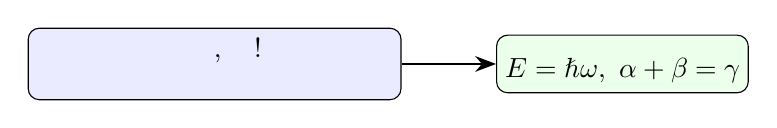
\begin{tikzpicture}[>=Stealth,every node/.style={align=center}]
  \node[draw,rounded corners,fill=blue!8,text width=4.5cm] (a) at (0,0) {Привет, мир!\\Геометрия и оптика};
  \node[draw,rounded corners,fill=green!8,right=1.2cm of a] (b) {\sffamily Научный рисунок\\\(E=\hbar\omega,\ \alpha+\beta=\gamma\)};
  \draw[->,line width=1pt] (a) -- (b);
\end{tikzpicture}
\end{document}
